\section{Simulazioni MIL}
\todo[inline]{I parametri usati in MIL e SIL per i controllori sono gli stessi}
\todo[inline]{Il controllori risultano iperattivi in MIL rispetto al SIL}

\subsection{PID}
\subsubsection{SNAKE}
\begin{figure}
	\centering
	\begin{subfigure}{0.45\textwidth}
		\centering
		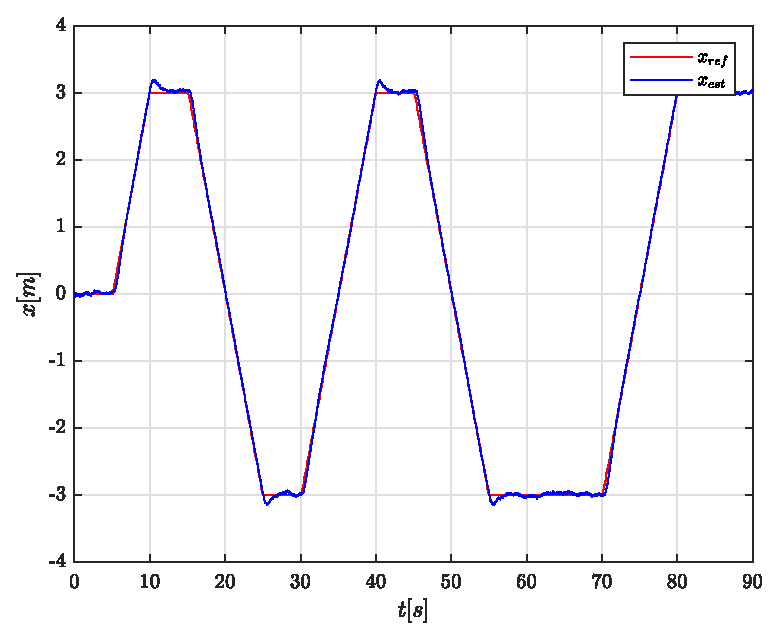
\includegraphics[width=1\textwidth]{Simulazioni/Figure/PID/SNAKE_MIL/PositionControlXPos}
		\caption{Controllo posizione lungo x}
	\end{subfigure}
	\hfill
	\begin{subfigure}{0.45\textwidth}
		\centering
		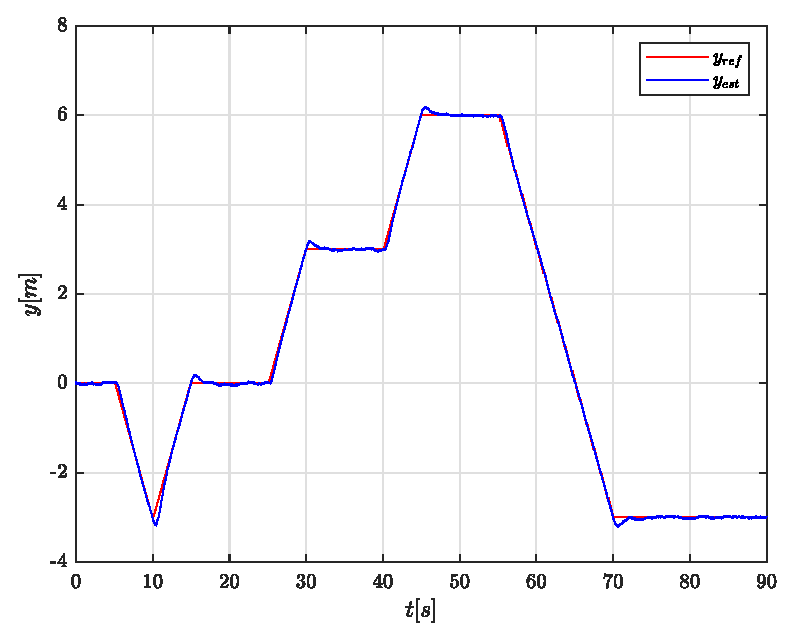
\includegraphics[width=1\textwidth]{Simulazioni/Figure/PID/SNAKE_MIL/PositionControlYPos}
		\caption{Controllo posizione lungo y}
	\end{subfigure}
	\\
	\begin{subfigure}{0.45\textwidth}
		\centering
		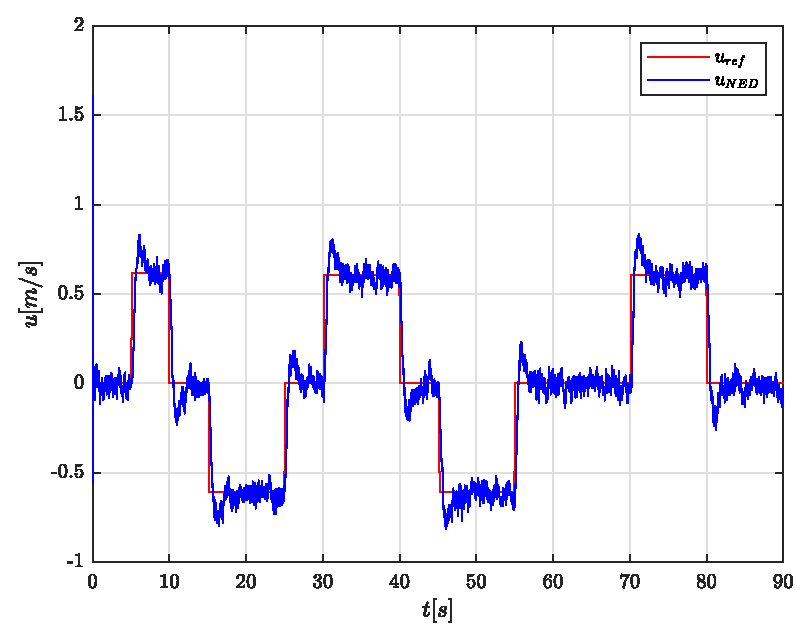
\includegraphics[width=1\textwidth]{Simulazioni/Figure/PID/SNAKE_MIL/PositionControlXVel}
		\caption{Controllo velocità lungo x}
	\end{subfigure}
	\hfill
	\begin{subfigure}{0.45\textwidth}
		\centering
		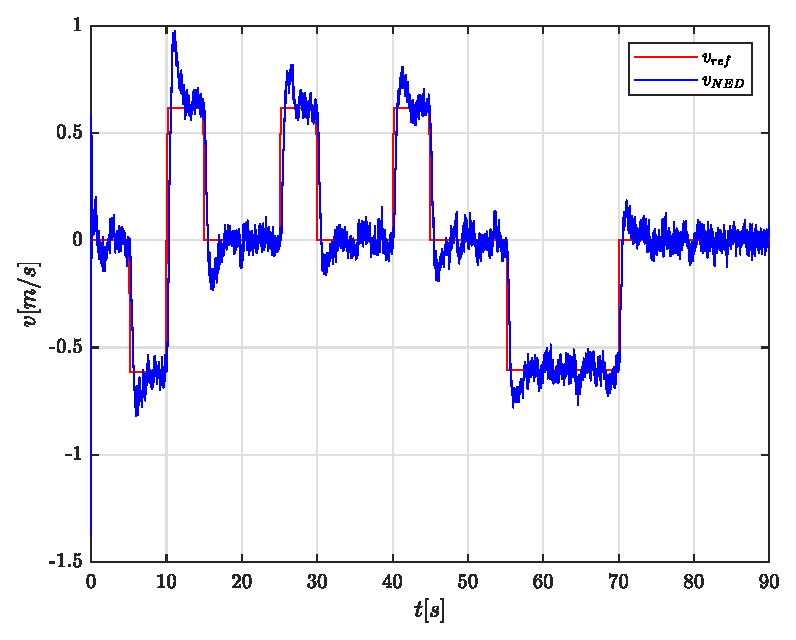
\includegraphics[width=1\textwidth]{Simulazioni/Figure/PID/SNAKE_MIL/PositionControlYVel}
		\caption{Controllo velocità lungo y}
	\end{subfigure}
	\caption{Risposta nella simulazione MIL in posizione con controllore interno PID al comando SNAKE}
\end{figure}

\begin{figure}
	\centering
	\begin{subfigure}{0.45\textwidth}
		\centering
		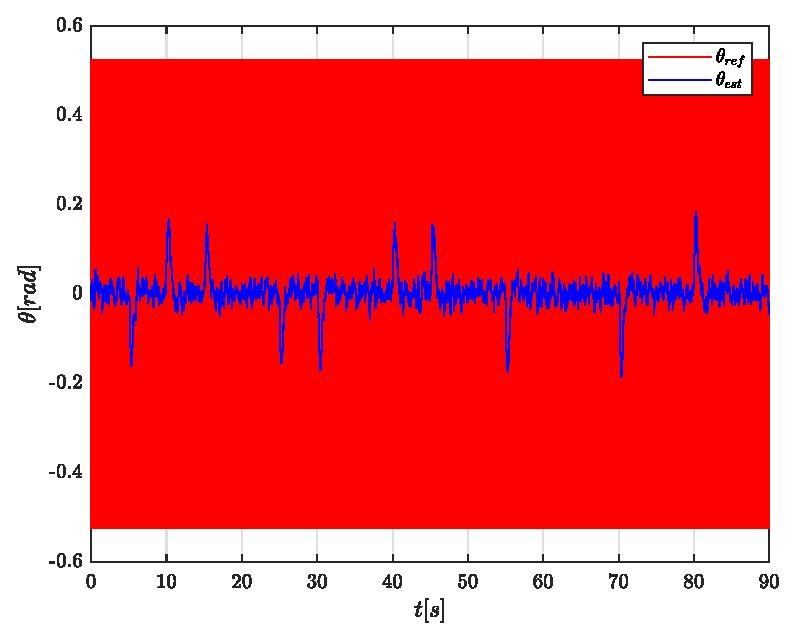
\includegraphics[width=1\textwidth]{Simulazioni/Figure/PID/SNAKE_MIL/AttitudeControlPitch}
		\caption{Controllo beccheggio}
	\end{subfigure}
	\hfill
	\begin{subfigure}{0.45\textwidth}
		\centering
		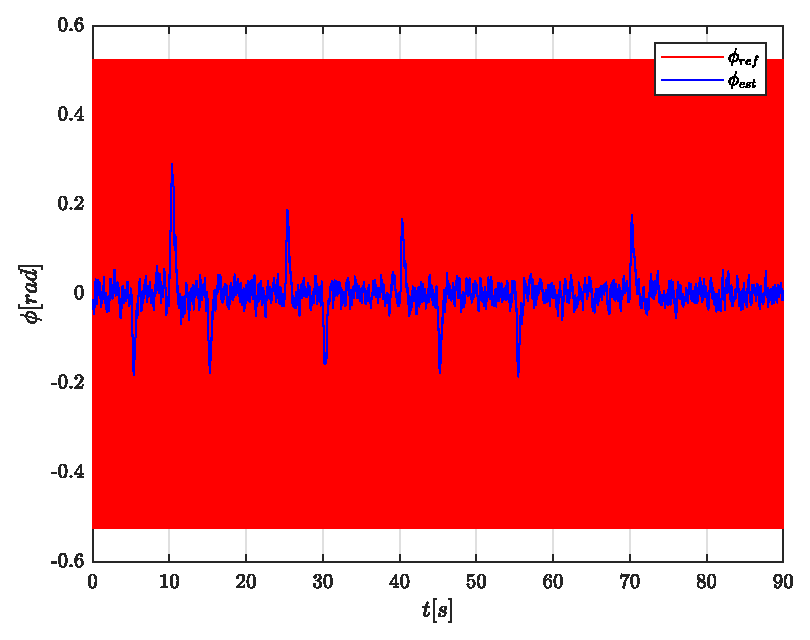
\includegraphics[width=1\textwidth]{Simulazioni/Figure/PID/SNAKE_MIL/AttitudeControlRoll}
		\caption{Controllo rollio}
	\end{subfigure}
	\hfill
	\begin{subfigure}{0.45\textwidth}
		\centering
		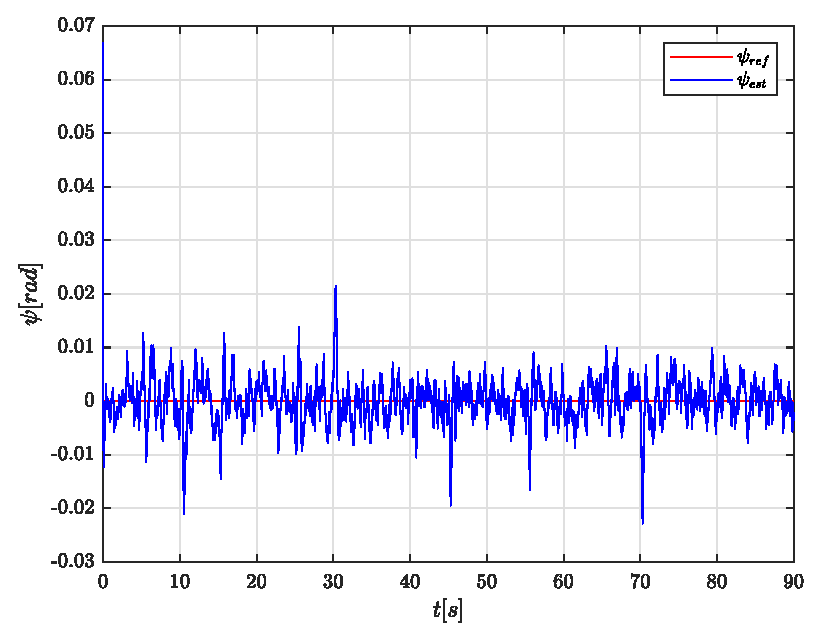
\includegraphics[width=1\textwidth]{Simulazioni/Figure/PID/SNAKE_MIL/AttitudeControlYaw}
		\caption{Controllo imbardata}
	\end{subfigure}
	\caption{Risposta dell' assetto nella simulazione MIL con controllore interno PID al comando SNAKE}
\end{figure}


\begin{figure}
	\centering
	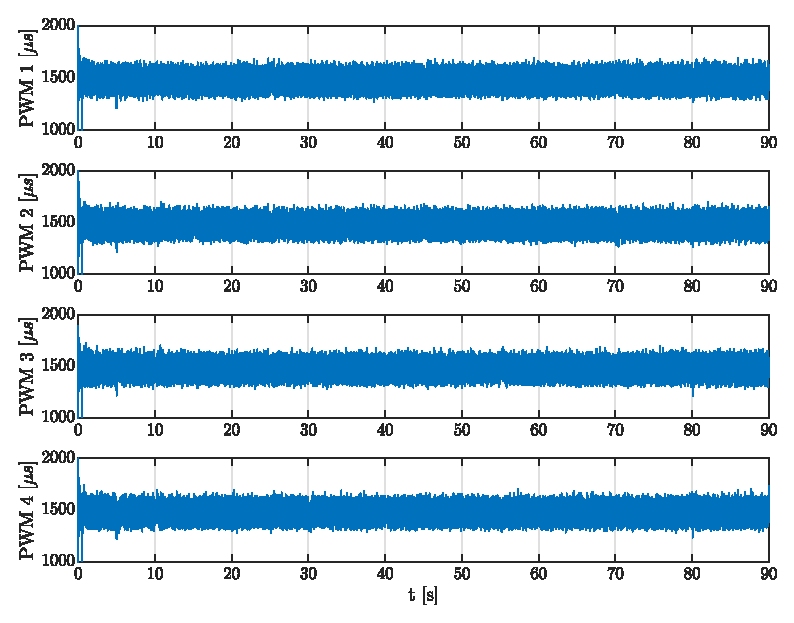
\includegraphics[width=0.5\textwidth]{Simulazioni/Figure/PID/SNAKE_MIL/PWM}
	\caption{Segnali PWM nella simulazione MIL del controllore PID al segnale SNAKE}
\end{figure}
\begin{figure}
	\centering
	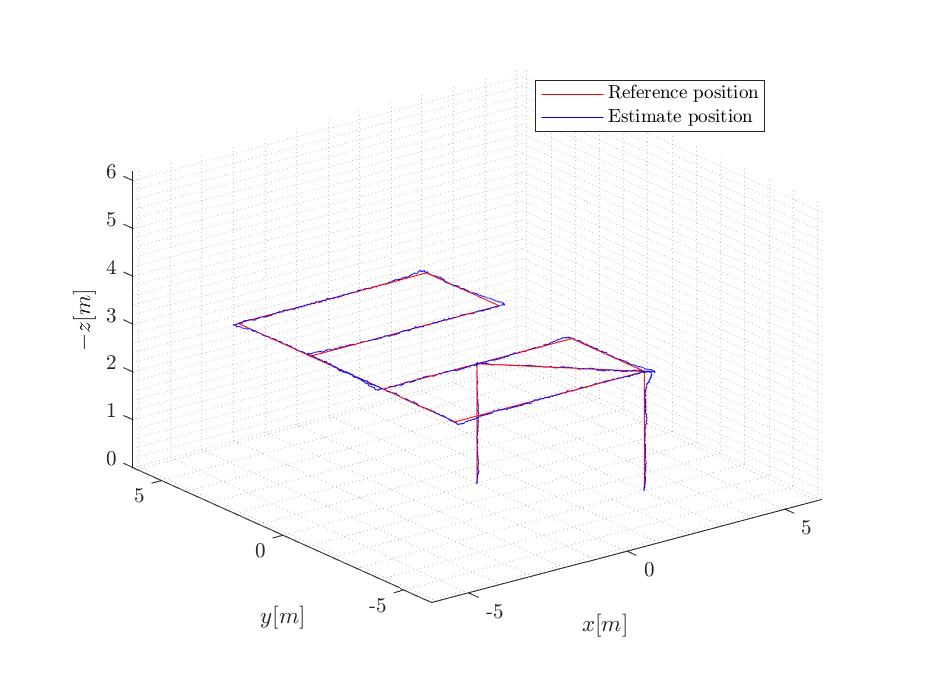
\includegraphics[width=1\textwidth]{Simulazioni/Figure/PID/SNAKE_MIL/Trajectory}
	\caption{Traiettoria percorsa nella simulazione MIL con controllore PID al segnale SNAKE}
\end{figure}

\clearpage
\subsection{SMC}
\subsubsection{SNAKE}
\begin{figure}
	\centering
	\begin{subfigure}{0.45\textwidth}
		\centering
		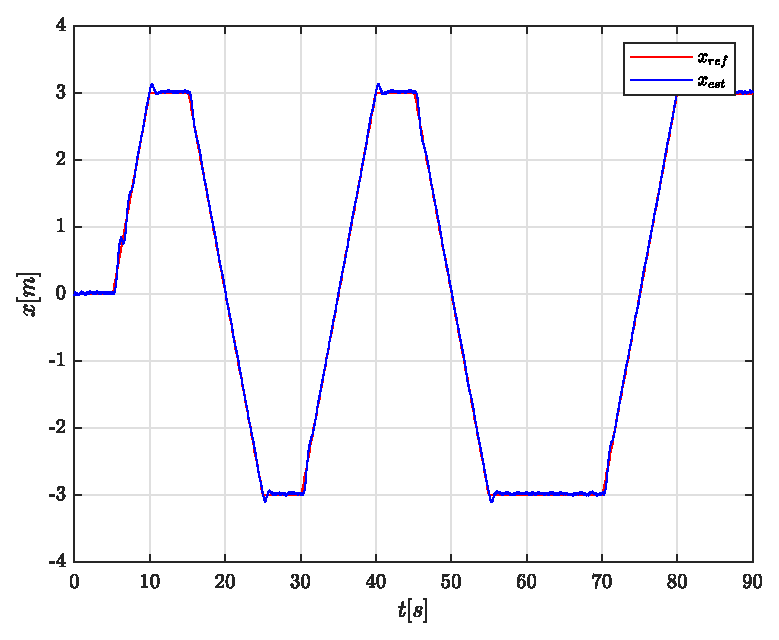
\includegraphics[width=1\textwidth]{Simulazioni/Figure/SMC/SNAKE_MIL/PositionControlXPos}
		\caption{Controllo posizione lungo x}
	\end{subfigure}
	\hfill
	\begin{subfigure}{0.45\textwidth}
		\centering
		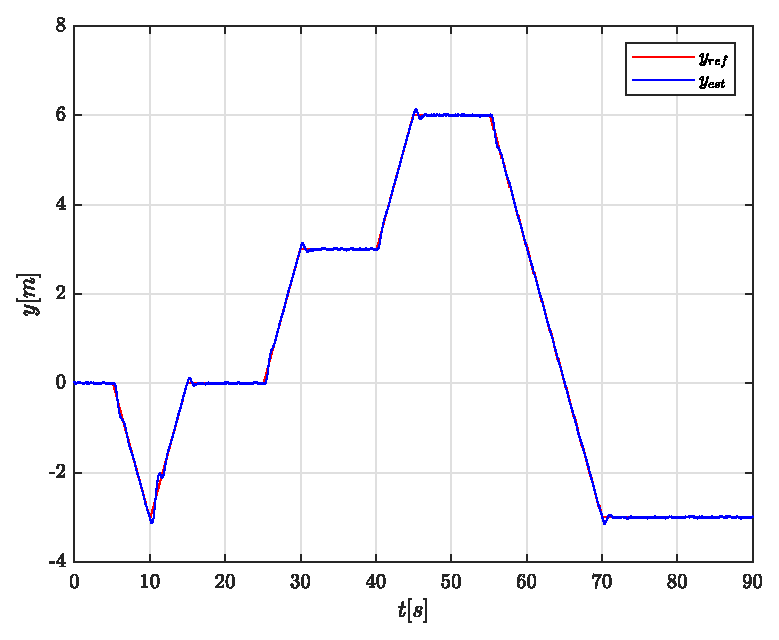
\includegraphics[width=1\textwidth]{Simulazioni/Figure/SMC/SNAKE_MIL/PositionControlYPos}
		\caption{Controllo posizione lungo y}
	\end{subfigure}
	\\
	\begin{subfigure}{0.45\textwidth}
		\centering
		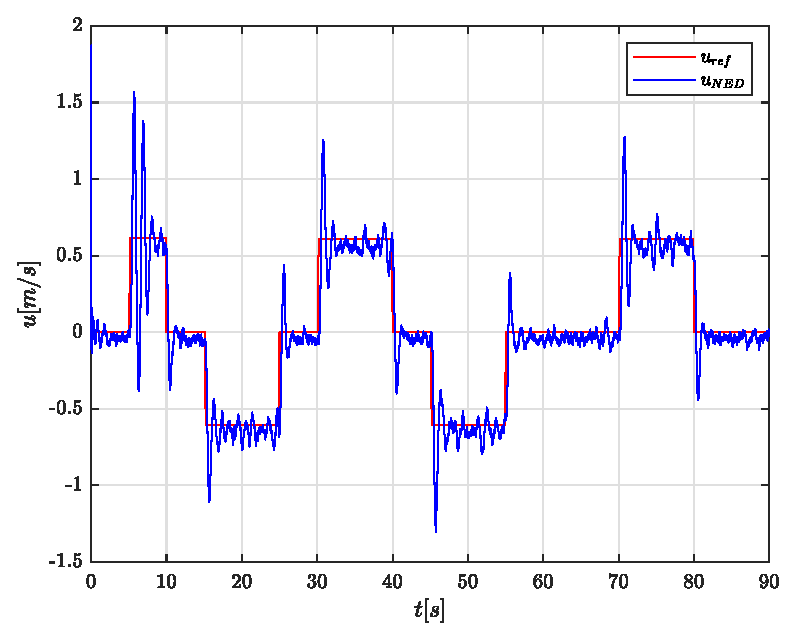
\includegraphics[width=1\textwidth]{Simulazioni/Figure/SMC/SNAKE_MIL/PositionControlXVel}
		\caption{Controllo velocità lungo x}
	\end{subfigure}
	\hfill
	\begin{subfigure}{0.45\textwidth}
		\centering
		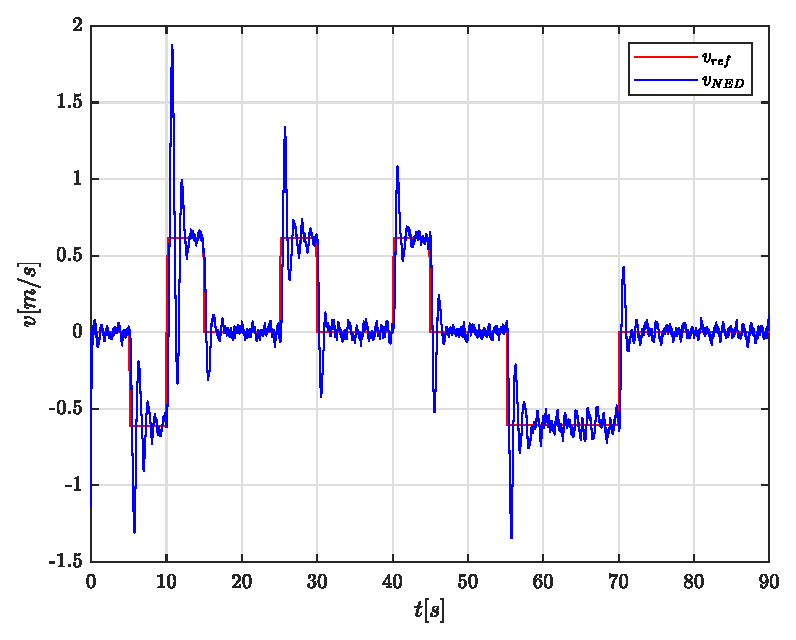
\includegraphics[width=1\textwidth]{Simulazioni/Figure/SMC/SNAKE_MIL/PositionControlYVel}
		\caption{Controllo velocità lungo y}
	\end{subfigure}
	\caption{Risposta in posizione nella simulazione MIL con controllore interno SMC al comando SNAKE}
\end{figure}

\begin{figure}
	\centering
	\begin{subfigure}{0.45\textwidth}
		\centering
		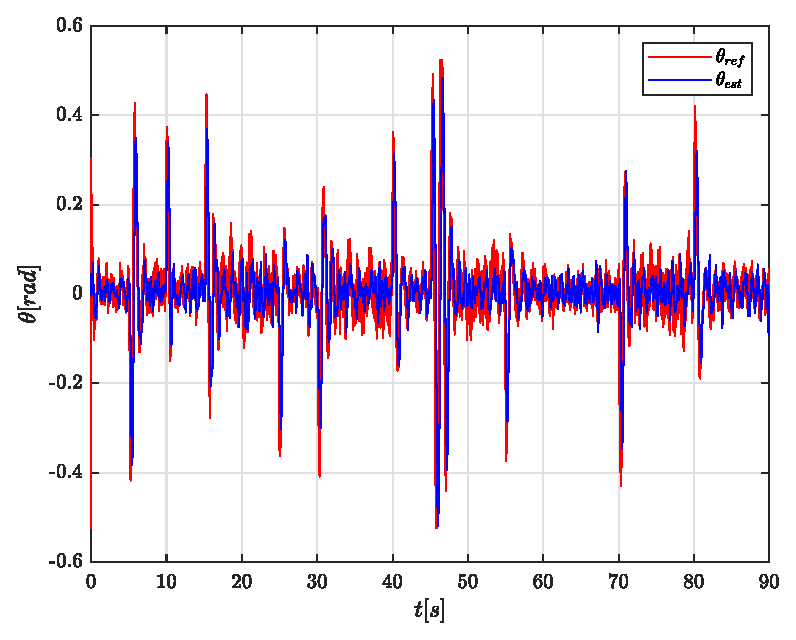
\includegraphics[width=1\textwidth]{Simulazioni/Figure/SMC/SNAKE_MIL/AttitudeControlPitch}
		\caption{Controllo beccheggio}
	\end{subfigure}
	\hfill
	\begin{subfigure}{0.45\textwidth}
		\centering
		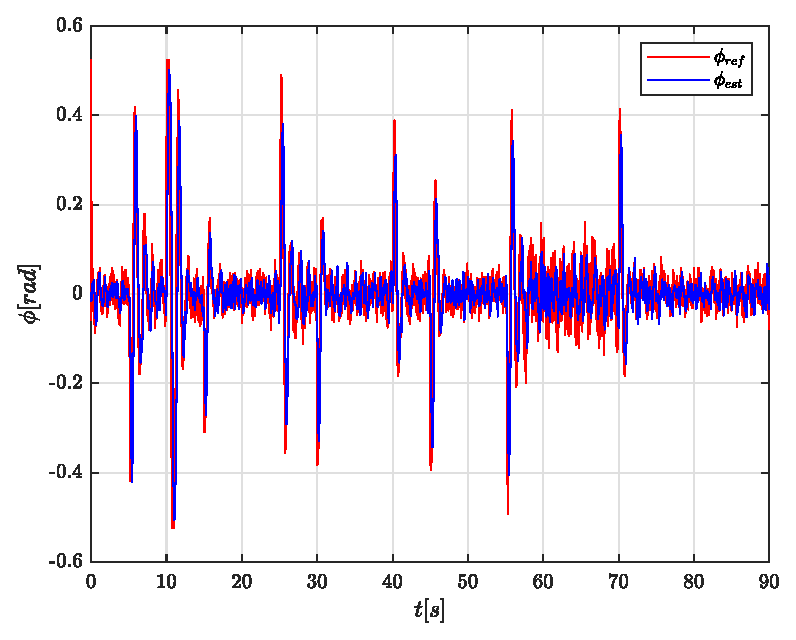
\includegraphics[width=1\textwidth]{Simulazioni/Figure/SMC/SNAKE_MIL/AttitudeControlRoll}
		\caption{Controllo rollio}
	\end{subfigure}
	\hfill
	\begin{subfigure}{0.45\textwidth}
		\centering
		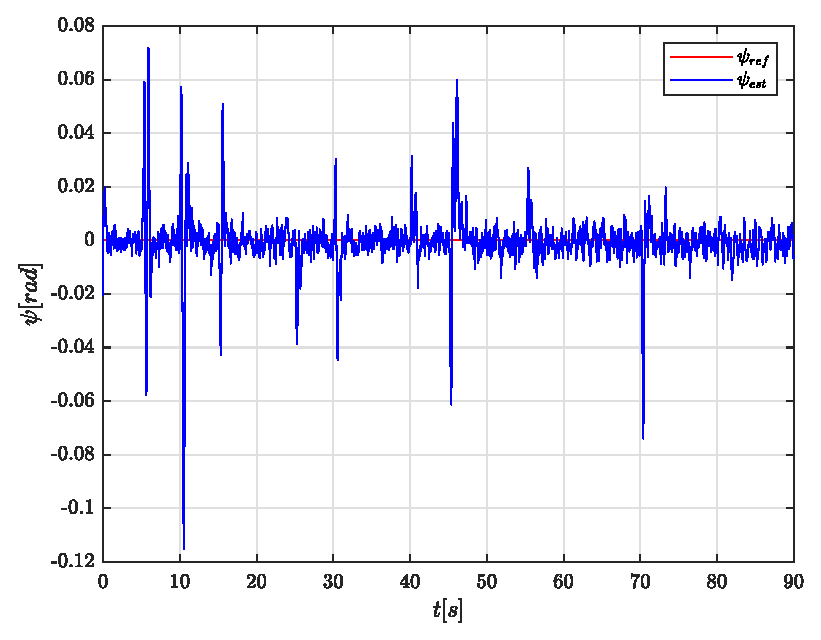
\includegraphics[width=1\textwidth]{Simulazioni/Figure/SMC/SNAKE_MIL/AttitudeControlYaw}
		\caption{Controllo imbardata}
	\end{subfigure}
	\caption{Risposta dell' assetto nella simulazione MIL con controllore interno SMC al comando SNAKE}
\end{figure}


\begin{figure}
	\centering
	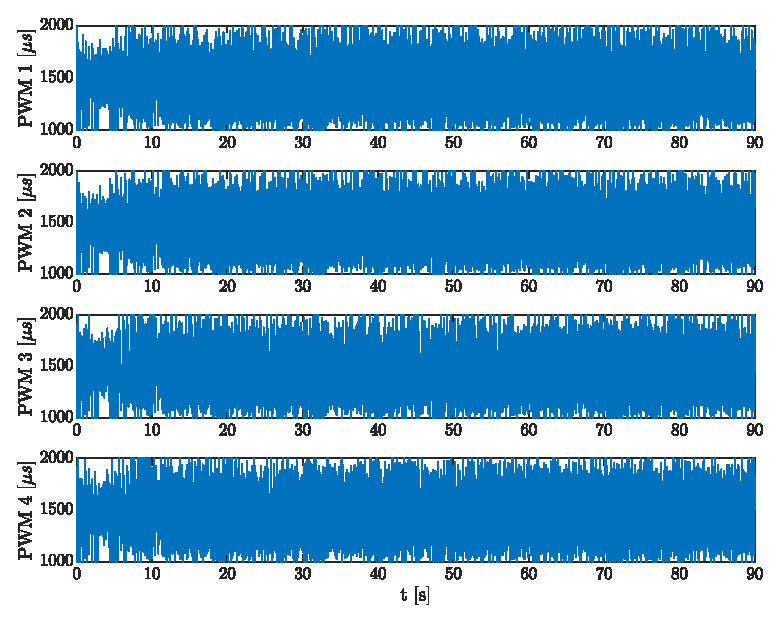
\includegraphics[width=0.5\textwidth]{Simulazioni/Figure/SMC/SNAKE_MIL/PWM}
	\caption{Segnali PWM del controllore SMC al segnale SNAKE}
\end{figure}
\begin{figure}
	\centering
	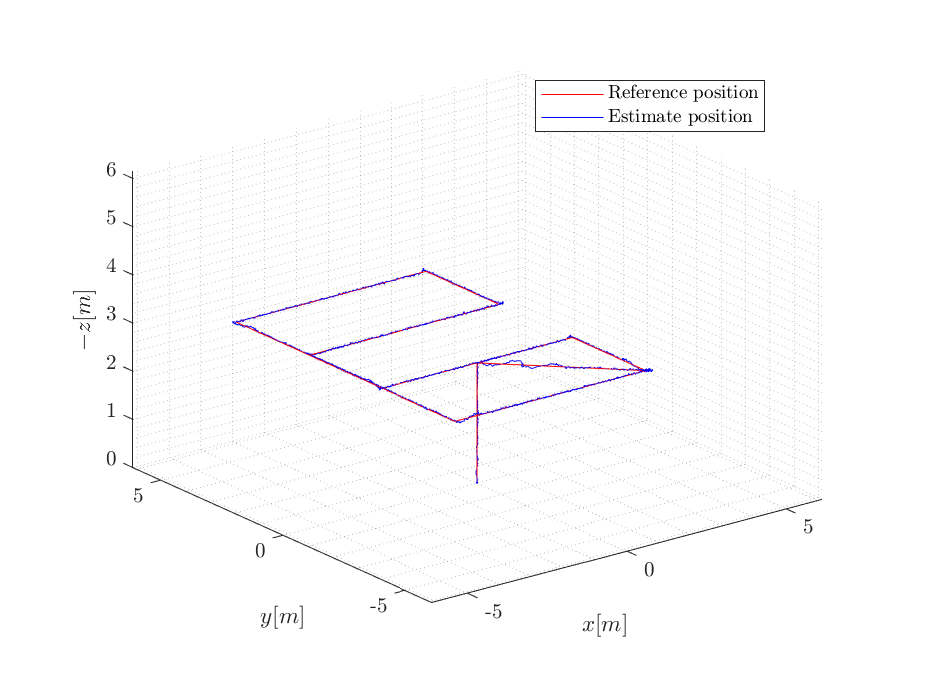
\includegraphics[width=1\textwidth]{Simulazioni/Figure/SMC/SNAKE_MIL/Trajectory}
	\caption{Traiettoria percorsa con controllore SMC nella simulazione MIL al segnale SNAKE}
\end{figure}
\subsection{Confronto}
\todo[inline]{Confronto tra MIL e SIL per il segnale SNAKE}
\todo[inline]{Il controllore SMC risulta più robusto. Il Controllore PID non si sarebbe mai ottenuto partendo dal MIL perchè in quel tipo di simulazione ha una risposta pessima. Importanza della SIL per valutare l'effetto introdotto dall'implementazione software per correggere i parametri di reogalzione trovati in MIL}
